\documentclass[border=4pt]{standalone}
\usepackage{tikz}
\usetikzlibrary{arrows.meta}
\definecolor{ink}{HTML}{2A2620}
\definecolor{violet}{HTML}{5A1BA6}
\definecolor{terracotta}{HTML}{A03A2C}
\definecolor{sage}{HTML}{8AA08A}
\definecolor{inkfaint}{HTML}{7A6F62}
\begin{document}
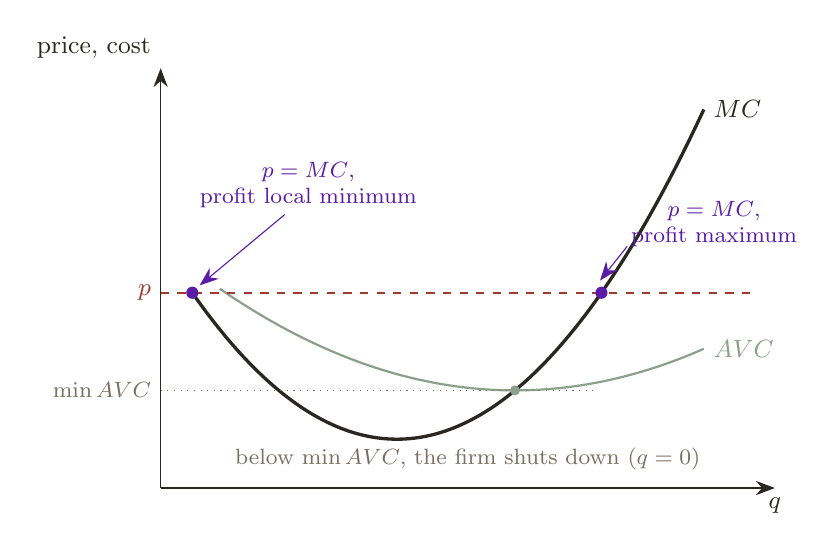
\begin{tikzpicture}[x=1.5cm,y=0.62cm,>={Stealth[length=2.4mm]},font=\small]
  % axes
  \draw[->,ink] (0,0) -- (5.2,0) node[below]{$q$};
  \draw[->,ink] (0,0) -- (0,8.6) node[above left]{price, cost};
  % marginal cost: q^2 - 4q + 5
  \draw[ink,very thick,domain=0.25:4.6,samples=120,smooth,variable=\q]
     plot (\q,{(\q)*(\q) - 4*(\q) + 5});
  \node[ink,right] at (4.6,{4.6*4.6-4*4.6+5}) {$MC$};
  % average variable cost: q^2/3 - 2q + 5
  \draw[sage,thick,domain=0.5:4.6,samples=120,smooth,variable=\q]
     plot (\q,{(\q)*(\q)/3 - 2*(\q) + 5});
  \node[sage,right] at (4.6,{4.6*4.6/3-2*4.6+5}) {$AVC$};
  % price line p = 4
  \draw[terracotta,thick,dashed] (0,4) -- (5,4);
  \node[terracotta,left] at (0,4) {$p$};
  % the two roots of p = MC
  \fill[violet] (0.268,4) circle (2.2pt);
  \fill[violet] (3.732,4) circle (2.2pt);
  \node[violet,align=center,font=\footnotesize] at (1.25,6.2) {$p=MC$,\\profit local minimum};
  \draw[violet,->] (1.05,5.6) -- (0.33,4.15);
  \node[violet,align=center,font=\footnotesize,anchor=west] at (3.9,5.4) {$p=MC$,\\profit maximum};
  \draw[violet,->] (3.95,4.95) -- (3.72,4.25);
  % shutdown price = min AVC
  \draw[inkfaint,dotted] (0,2) -- (3.7,2);
  \fill[sage] (3,2) circle (1.8pt);
  \node[inkfaint,left,font=\footnotesize] at (0,2) {$\min AVC$};
  \node[inkfaint,font=\footnotesize] at (2.6,0.6) {below $\min AVC$, the firm shuts down ($q=0$)};
\end{tikzpicture}
\end{document}
